\section{Grundlagen des maschinellen Lernens} \label{sec:Grundlagen ML}
Traditionelle Computerprogramme bestehen aus einer Abfolge von Befehlen, welche dem Computer Schritt für Schritt erklären, was er tun soll. \glsdisp{ML}{Lern-Algorithmen} sind in der Lage eigenständig herauszufinden, was sie tun sollen. \Gls{ML} hat seine Anfänge in den 1950er Jahren. Seither wurde eine Vielzahl an Ansätzen entwickelt, um Maschinen Lernfähigkeit zu verleihen. Diese reichen von einfachen statistischen Modellen bis hin zu komplexen neuronalen Netzen. Heutzutage ist \gls{ML} fester Bestandteil unseres Alltags. Sei es durch Empfehlungsalgorithmen beim Online-Shopping, durch Spam-Filter für das E-Mail Postfach, in der Überwachung von öffentlichen Räumen durch \gls{MOT} oder durch den neusten Trend: Large Language Modells wie \textit{ChatGPT} \cite{Domingos.2015, Liu.2023}. Die Geschichte des \gls{ML} zeigt, dass für Computer oftmals die Aufgaben am herausforderndsten sind, welche Menschen intuitiv bewältigt werden können. Es ist schwierig einem Computer den Lösungsweg für solche Aufgaben zu erklären \cite{Goodfellow.2016}. \par

In \cite{Mitchell.1997} wird \gls{ML} beschrieben, als ein Lernprozess, welcher ein Computer automatisch durchführt. Es wird wie folgt definiert: Ein Computerprogramm ist Lernfähig, wenn es sich durch Erfahrung \(E\) in seiner Performance \(P\) im Bezug auf die Bewältigung einer Aufgabe \(A\) verbessert. In einem Beispiel möchte ein Autohändler den Verkaufswert von Autos schätzen. Dazu muss er zunächst auswählen, welche Eigenschaften eines Autos er für die Schätzung nutzen möchte. Er entscheidet sich für die Anzahl der gefahrenen Kilometer und das Alter des Autos. Solche Eigenschaften werden \gls{Feature}[s] genannt. \gls{Feature}[s] sind Merkmale, welche Informationen zur Bewältigung der Aufgabe \(A\) beisteuern. Die \gls{Feature}[s] werden in einer \gls{Datenmatrix} \(\nommat{X}\) angeordnet. Bezogen auf das Beispiel beinhalten die Spalten in \(\nommat{X}\) die Werte der gefahrenen Kilometer und des Alters der Autos. Die Zeilen von \(X\) beinhalten die \gls{Feature}[s] zu jeweils einem Auto. Neben der \gls{Datenmatrix} benötigen viele Modelle noch einen \gls{Zielvektor} \(\nomvec{y}\). Dieser Beinhaltet die Ziel-Werte für die Aufgabe A. Im Beispiel ist jedes Element \(\nomvec{y}_i\) der Wert eines Autos. Jede Reihe \(\nommat{X}_{i,:}\) beinhaltet die Informationen zu der Anzahl der gefahrenen Kilometer und des Alters von einem spezifischen Auto. Aus diesem Grund wird eine Zeile \(\nommat{X}_{i,:}\) auch \gls{Featurevektor} genannt. Das Element \(\nomvec{y}_i\) ist der Wert für den dieses spezifische Auto verkauft wurde. Zusammen bilden \(\nommat{X}\) und \(\nomvec{y}\) einen Datensatz. Dieser Datensatz ist die Erfahrung \(E\) mit dessen Hilfe das Programm lernen soll. Hat der Autohändler \(N=20\) Erfahrungswerte so ist der Datensatz Aufgebaut aus \(N\) Datenpunkten \(D = \{(\nommat{X}_{i,:}, \nomvec{y}_i)\}_{i}^{N}\) \cite{Goodfellow.2016, Burkov.2019, ShalevShwartz.2014}. Die Tabelle \ref{tab:BspMLAuto} zeigt den Aufbau des Datensatzes aus dem Beispiel. 


\begin{table}
    \centering
    \begin{tabular}{|r|r|r|}
     \hline
        Verkaufswert in €   & gefahrene Kilometer   & Alter in Jahren\\
     \hline
        10200               & 52000                 & 5             \\
     \hline
        7100                & 140000                & 12            \\
     \hline
        \vdots              & \vdots                & \vdots        \\
     \hline
         23800              & 25000                 & 2             \\
      \hline
    \end{tabular}
    \caption{Aufbau des Datensatzes für das Beispiel der Schätzung von Verkaufswerten von Autos. Die Spalte \textit{Verkaufswerte} entspricht \(\nomvec{y}\). Die Spalten \textit{gefahrene Kilometer} und \textit{Alter in Jahren} bilden \(\nommat{X}\). }
    \label{tab:BspMLAuto}
\end{table}

Damit ist die Aufgabe \(A\) und die Erfahrung \(E\) für das Beispiel definiert. 

\begin{itemize}
    \item A: Schätzung des Verkaufswerts von Autos.
    \item E: Datensatz aus den \gls{Feature}[s] und den \glsdisp{Zielvektor}{Zielwerten}.
\end{itemize}

\begin{figure}[htb]
    \centering
    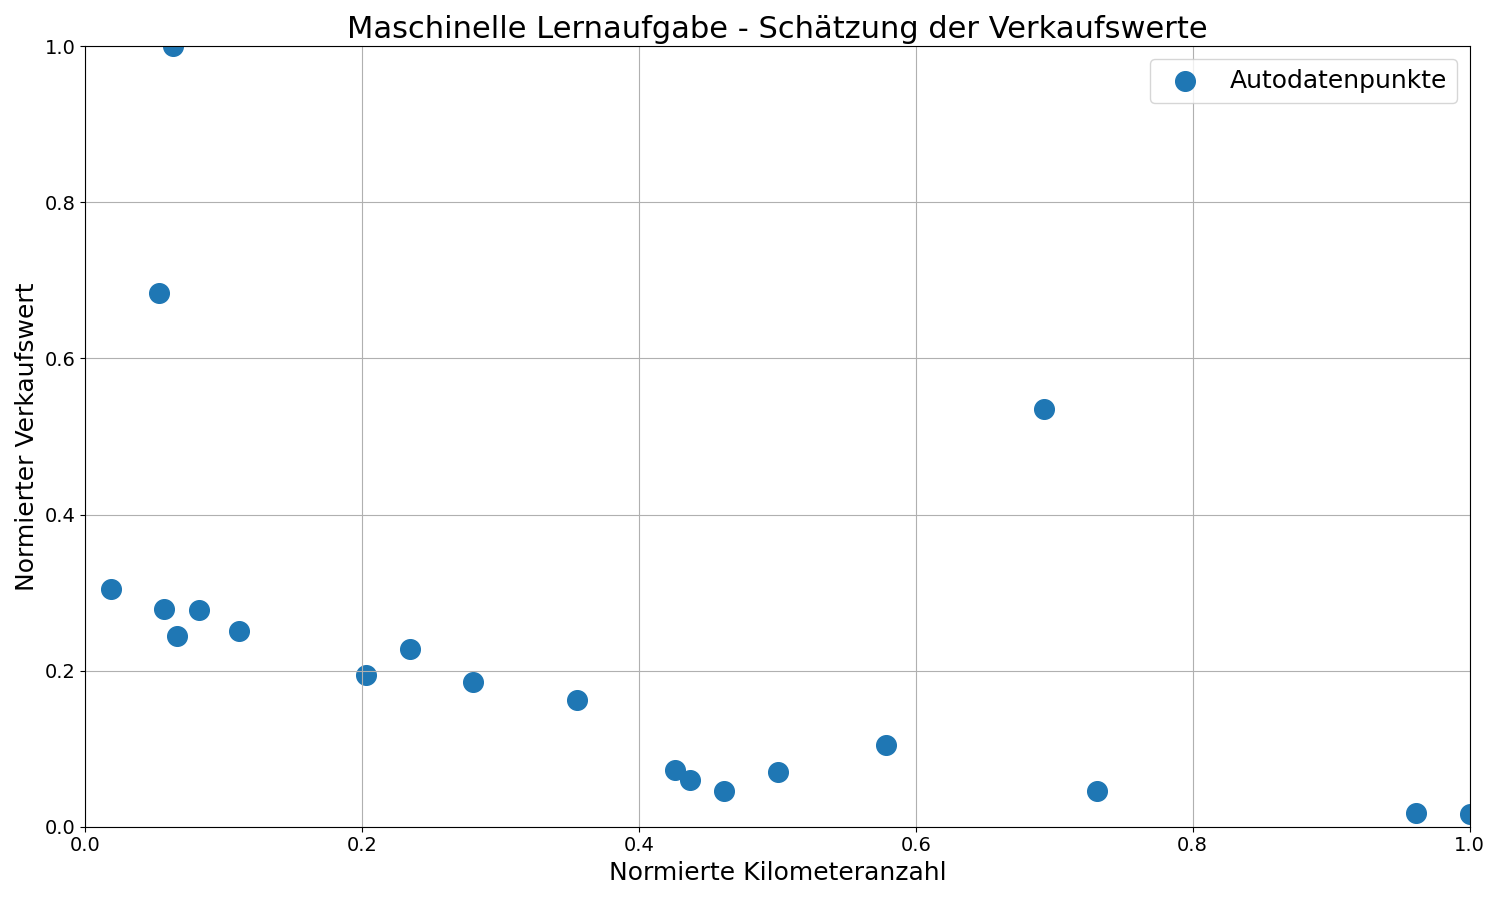
\includegraphics[width=0.9\textwidth]{img/Autohändlerbsp/Schätzung der Verkaufswerte.png}
    \caption[Beispiel einer maschinellen Lernaufgabe.]{Beispiel einer \glsdisp{ML}{maschinellen Lernaufgabe}. Schätzung vom Verkaufswerten von Autos. Auf der y-Achse ist der \glsdisp{Zielvektor}{Zielwert} dargestellt. Auf der y-Achse ist die \gls{Feature} \textit{Anzahl der gefahrenen Kilometer} abgebildet. Die Werte der Achsen sind normiert.}
    \label{fig:BspMLAuto}
\end{figure}


Die Abbildung \ref{fig:BspMLAuto} zeigt die die Punkte in \(D\) für den \glsdisp{Zielvektor}{Zielwert} und das \gls{Feature} \textit{Anzahl der gefahrenen Kilometer}. Um ein Lernfähiges Programm zu erhalten muss eine mathematische Repräsentation für die Bewältigung der Aufgabe \(A\) gefunden werden. Durch diese mathematische Repräsentation, ist die Performance \(P\) des Programms bewertbar \cite{Mitchell.1997}. Ein einfacher Algorithmus für \gls{ML} ist die lineare Regression. Diese wird für das Problem des Autohändlers durchgeführt. Für eine linearen Regression wird die Repräsentation aus \autoref{eq:linReg} für die Lösung von \(A\) gewählt.

\begin{equation}
    \label{eq:linReg}
    \hat{y}(\nomvec{w}, \nomvec{x}) =  \nomvecT{w}\nomvec{x} = \nomvec{w}_1\nomvec{x}_1 + \nomvec{w}_2\nomvec{x}_2 + \dots + \nomvec{w}_n\nomvec{x}_n
\end{equation}

Der vom Programm geschätzte Wert eines Autos ist \(\hat{y}(\nomvec{w}, \nomvec{x})\). Der Vektor \(\nomvec{x}\) ist ein \gls{Featurevektor} und er beinhaltet die Werte der \gls{Feature}[s] zu einem Auto. Der Vektor \(\nomvecT{w}\) beinhaltet Gewichte für die \gls{Feature}[s]. Für die Schätzung von \(\hat{y}(\nomvec{w}, \nomvec{x})\) wird somit jeder \gls{Feature}[wert] \(\nomvec{x}_i\) mit einem Parameter \(\nomvecT{w}_i\) gewichtet, welcher den Einfluss des \gls{Feature}[s] \(\nomvec{x}_i\) beschreibt \cite{Goodfellow.2016}. Die Gewichte \(\nomvecT{w}\) werden \gls{Modellparameter} genannt. Allgemein ausgedrückt sind \gls{Modellparameter} das, was ein Programm bei einem \gls{Modelltraining}{Trainingsprozess} versucht zu lernen \cite{Zheng.2015}. \par

Mit dieser mathematischen Repräsentation lässt sich eine Formulierung zur Beurteilung der Performance \(P\) finden. Diese ist mit Hilfe der Erfahrung \(E\) zu ermitteln. Für eine Probe \(\nommat{X}_{i:}\) aus \(\nommat{X}\) lässt sich mit der linearen Regression ein Schätzwert \(\hat{y}(\nomvec{w}, \nommat{X}_{i:})\) berechnen. Der Fehler des Programms ist über die Differenz zum echten Wert \(\nomvec{y}_i\) bestimmbar. Um die Performance \(P\) des Modells zu bewerten wird der  \glsdisp{MSE}{mittlere quadratische Fehler (MSE)} von allen Proben \(N\) im Datensatz \(D\) berechnet. Die Berechnung des \gls{MSE} ist in der \autoref{eq:MSE} zu sehen \cite{Goodfellow.2016, Burkov.2019}.

\begin{equation}
    \label{eq:MSE}
    MSE = \frac{1}{N} \sum_{i=1}^{N} (\hat{y}_i(\nomvec{w}, \nommat{X}_{i:}) - \nomvec{y}_i)_i^2
\end{equation}

Die Formulierung \((\hat{y}_i(\nomvec{w}, \nommat{X}_{i:}) - \nomvec{y}_i)^2\) wird als \gls{Verlustfunktion} bezeichnet. Jedes Modell des \glsdisp{ML}{maschinellen Lernens} besitzt ein \gls{Verlustfunktion}. Die in der \autoref{eq:MSE} verwendete \gls{Verlustfunktion} wird als quadratische \gls{Verlustfunktion} bezeichnet. Der \gls{MSE} ist hier eine \gls{Zielfunktion} für ein Optimierungsproblem. Der \gls{MSE} soll minimal werden. Dies ist in der \autoref{eq:minMSE} formuliert \cite{Goodfellow.2016, Burkov.2019}.

\begin{equation}
    \label{eq:minMSE}
    \underset{w}{\arg\min} \frac{1}{N} \sum_{i=1}^{N} (\hat{y}_i(\nomvec{w}, \nommat{X}_{i:}) - \nomvec{y}_i)_i^2
\end{equation}

Die Lösung von der \autoref{eq:minMSE} resultiert in optimalen Gewichten \(\nomvec{w}\), um \(\hat{y}(\nomvec{w}, \nomvec{x})\) möglichst genau zu Schätzen. Das Lösen der \autoref{eq:minMSE} ist der \glsdisp{ML}{Lernprozess} des Programms. Dieser wird mit einer Optimierungsroutine umgesetzt. Häufig verwendet wird das \gls{Gradientenverfahren}. Bei diesem wird wie folgt vorgegangen. Alle Parameter \(\nomvec{w}^{(t)}\) erhalten einen initial Wert für den Startzeitpunkt \(t=1\), bspw. \(\nomvec{w}_i^{(1)}=0 \forall i\). Für die \gls{Zielfunktion} wird der Gradient berechnet \(\nabla MSE(\nomvec{w}^{(t)})\). Iterativ wird nun in Richtung des steilsten Abstieges des Gradienten gegangen. Da der Gradient in Richtung des steilsten Anstieges zeigt, wird in die negative Richtung des Gradienten gegangen. Die Werte von \(\nomvec{w}\) werden bei jedem Schritt aktualisiert \cite{Mitchell.1997, Goodfellow.2016, ShalevShwartz.2014}. Dies zeigt die Formulierung \ref{eq:GradDecentUpdateW}.

\begin{equation}
    \label{eq:GradDecentUpdateW}
    \nomvec{w}^{(t+1)} \leftarrow \nomvec{w}^{(t)} - \eta\nabla MSE(\nomvec{w}^{(t)})
\end{equation}

Der Parameter \(\eta\) wird dabei als Lernrate bezeichnet. Die Lernrate bestimmt die Schrittgröße, welche bei jeder Iteration in Richtung des steilsten Abstiegs gegangen wird \cite{Mitchell.1997}. Die Lernrate ist vom Anwender einzustellen. Parameter, welche vom Anwender festzulegen sind werden \gls{Hyperparameter} gennant. Sie sind nicht zu verwechseln mit den \gls{Modellparameter}[n] \cite{Zheng.2015}. Bei einem Minimum gilt \(\nabla MSE(\nomvec{w}^{(t)}) = 0\). Verändern sich die Werte von \(\nomvec{w}^{(t)}\) durch weiterer Iterationen nicht mehr, wurde ein Minimum gefunden \cite{Goodfellow.2016, Burkov.2019}. Die Abbildung \ref{fig:GradDecentBsp} veranschaulicht die Suche des Minimums durch das \gls{Gradientenverfahren}.

\begin{figure}[htb]
    \centering
    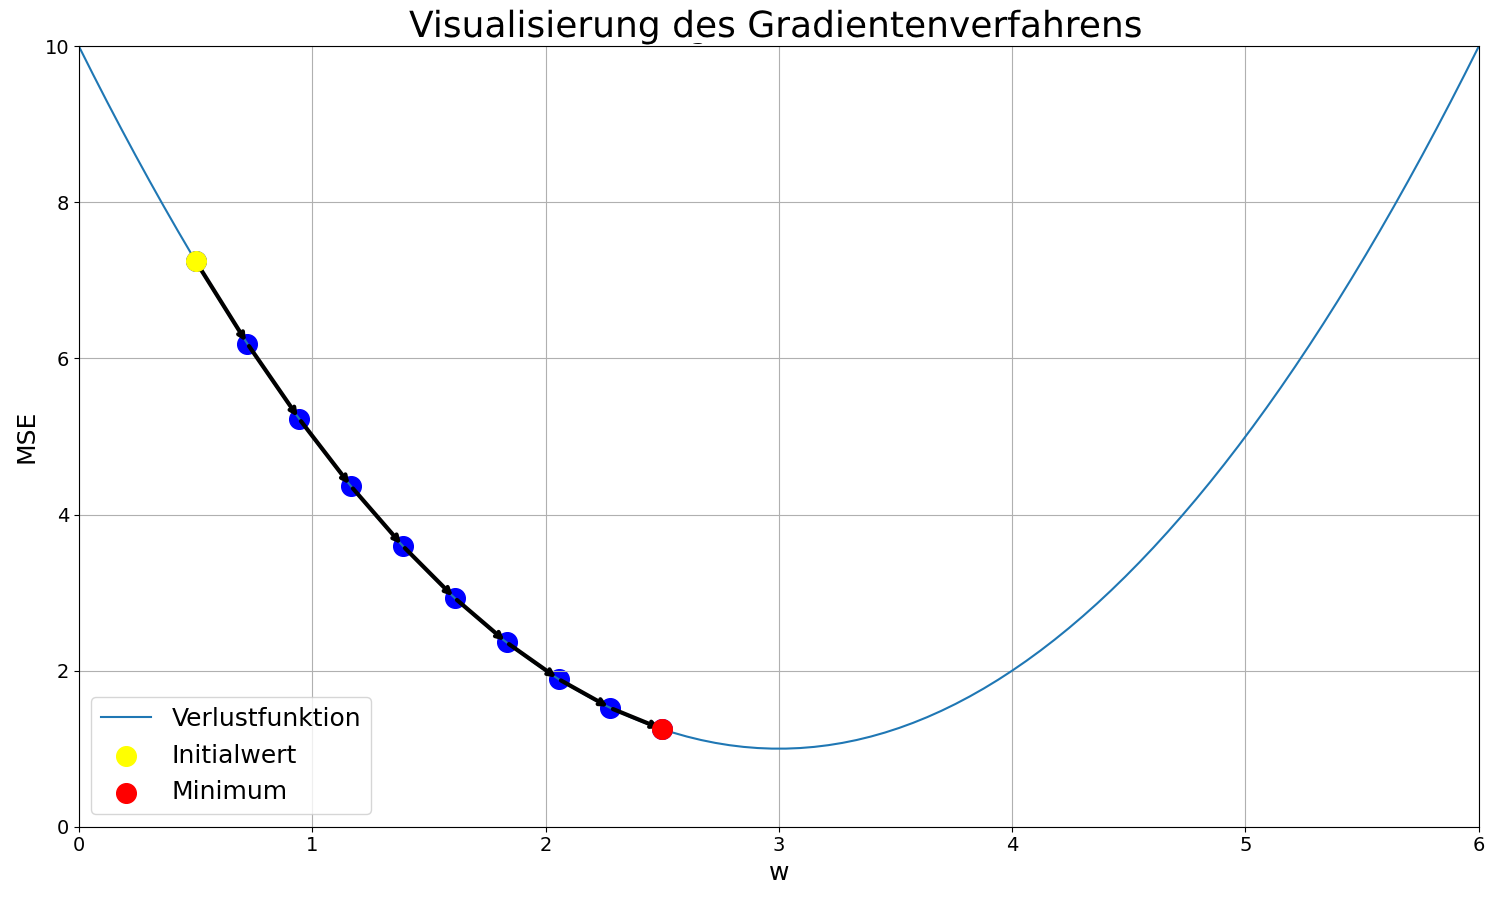
\includegraphics[width=0.9\textwidth]{img/Plots/Gradientverfahren.png}
    \caption[Vorgehen des Gradientenverfahrens.]{Vorgehen des Gradientenverfahrens. Iterativ wird das Minimum des Optimierungsproblems gesucht. Gestartet wird bei einem Initialwert. Ändert sich das Minimum nur noch geringfügig, wird der Wert als Lösung genommen.}
    \label{fig:GradDecentBsp}
\end{figure}

Mit diesem vorgehen ist auch das Beispiel des Autohändlers lösbar. Um das Beispiel anschaulich zu halten, wird das Modell der lineare Regression aus der \autoref{eq:linReg} nur mit dem \gls{Feature} der Anzahl der gefahrenen Kilometer trainiert. Die Abbildung \ref{fig:BspMLAutoMitReg} zeigt die gleichen Datenpunkte dar, wie die Abbildung \ref{fig:BspMLAuto}, jedoch ist nun die resultierende Gerade \(\hat{y}(x)\) eingezeichnet. 

\begin{figure}[htb]
    \centering
    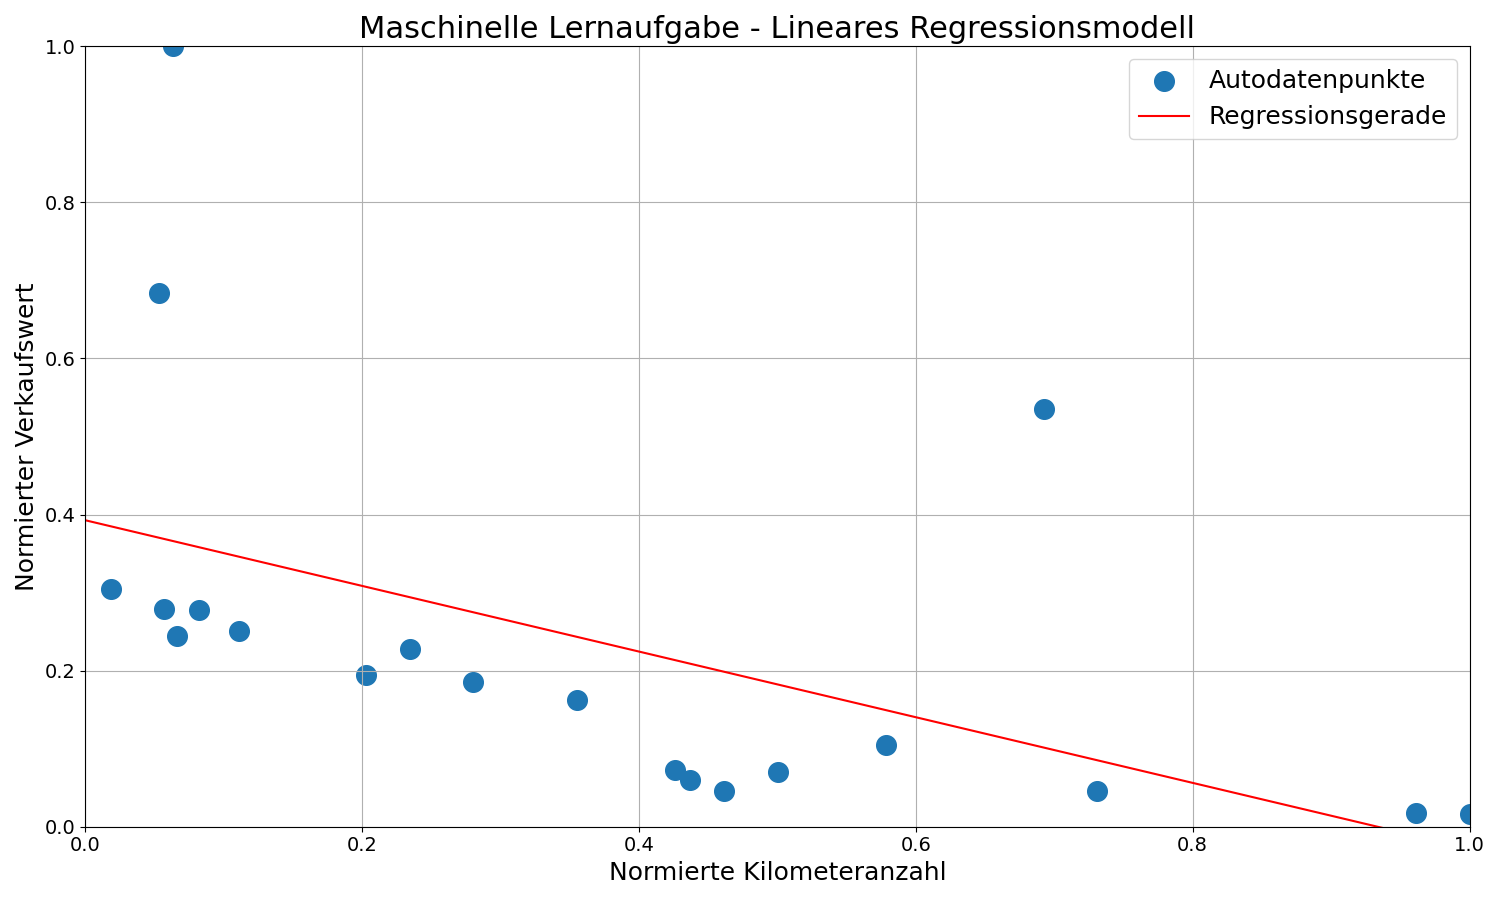
\includegraphics[width=0.9\textwidth]{img/Autohändlerbsp/Lineares Regressionsmodell.png}
    \caption[Beispiel einer linearen Regression von Autoverkaufswerten.]{Beispiel einer linearen Regression von Autoverkaufswerten. Die Datenpunkte stammen von verkauften Autos. Auf der y-Achse sind die Verkaufspreise dargestellt. Auf der x-Achse ist die Anzahl der gefahrenen Kilometer zu sehen. Beide Achsen sind normiert. Eingezeichnet ist eine Gerade. Die Gerade wurde durch eine lineare Regression ermittelt.}
    \label{fig:BspMLAutoMitReg}
\end{figure}

Das Beispiel der linearen Regression zeigt, dass sich die Bestandteile eines Algorithmus für \gls{ML} allgemein wie folgt zusammenfassen lassen \cite{Burkov.2019, Mitchell.1997, Goodfellow.2016}.

\begin{enumerate}
    \item \textbf{Definition einer Aufgabe:} Eine Aufgabe muss definiert werden, welche durch \gls{ML} gelöst werden soll. Für diese Aufgabe muss eine mathematische Repräsentation gefunden werden.
    \item \textbf{Definition einer \gls{Verlustfunktion}:} Um die Performance des Algorithmus zu bewerten, ist eine \gls{Verlustfunktion} zu definieren.
    \item \textbf{Definition einer \gls{Zielfunktion}:} Die \gls{Verlustfunktion} ist in ein Optimierungsproblem zu überführen, für welches eine \gls{Zielfunktion} zu formulieren ist.
    \item \textbf{Definition einer Optimierungsroutine:} Um das Optimierungsproblem der \gls{Zielfunktion} zu lösen wird ein Algorithmus benötigt, welcher das gesuchte Optimum findet. Für die Berechnung wird Erfahrung benötigt in Form eines Datensatzes.
\end{enumerate}


\subsection{Klassifizierung und Regression} \label{sec:ML klass und Reg}
Die Aufgaben, für welche \gls{ML} am häufigsten verwendet wird sind Regression und \gls{Klassifikation}. Im \autoref{sec:Grundlagen ML} wurde der Algorithmus der linearen Regression angewendet um ein Regressionsproblem zu lösen. Bei der Regression wird ein Zielwert \(\hat{y}(\nomvec{x}) \in \mathbb{R}\) geschätzt. Wobei \(\nomvec{x}\) der \gls{Feature}[vektor] einer Probe ist. Der Datensatz, mit welchem das Modell \glsdisp{Modelltraining}{trainiert} wird besteht aus einer \gls{Datenmatrix} \(\nommat{X}\), welche \gls{Feature}[werte] beinhaltet und einem \gls{Zielvektor} \(\nomvec{y}\), welcher die korrekten Zielwerte zu den Proben der \gls{Datenmatrix} beinhaltet. Für \(\nomvec{y}\) gilt ebenfalls \(\nomvec{y}_i \in \mathbb{R} \forall i \) \cite{Burkov.2019, ShalevShwartz.2014}. \par

Bei der \gls{Klassifikation} soll ein Modell unbekannte Proben einer Klasse zuordnen. Anstatt eines reelen Zielwerts soll für \(\hat{y}(\nomvec{x})\) eine Klassenzugehörigkeit geschätzt werden. Als Ergebnis vergibt ein \glsdisp{Klassifikation}{Klassifikator} einer Probe ein \gls{Label}, welches die Klassenzugehörigkeit deutlich macht. Der Vektor \(\nomvec{y}\) wird deshalb für \glsdisp{Klassifikation}{Klassifizierungsprobleme} meistens als \gls{Labelvektor} bezeichnet. Im folgenden wird der Begriff \gls{Zielvektor} als allgemeine Form verwendet. Ein klassisches Beispiel für ein \glsdisp{Klassifikation}{Klassifizierungsproblem} ist ein Spam-Filter für das E-Mail Postfach. Dieser ordnet neu eintreffende E-Mails entweder in die Klasse \textit{Kein Spam}, oder in die Klasse \textit{Spam} ein \cite{Burkov.2019}. \par

In dem Beispiel des Spam-Filters handelt es sich um binäre \gls{Klassifikation}. Das Modell muss nur zwischen zwei Klassen unterscheiden können. Ein weiteres Beispiel wäre ein Arzt, der seine Patienten in die Klassen \textit{Gesund} und \textit{Krank} einteilt. Es gibt jedoch auch Aufgaben bei denen zwischen mehr als zwei Klassen unterschieden werden muss. Solche Aufgaben werden als \gls{Mehrklassen Klassifizierung} bezeichnet. Ein Beispiel für \gls{Mehrklassen Klassifizierung} wäre wieder der Arzt, welcher für seine kranken Patienten von einem Modell direkt das passende Medikament empfohlen bekommen möchte. Die \gls{Datenmatrix} enthält \gls{Feature}[s] zu den Symptomen und Unverträglichkeiten der Patienten. Der \gls{Labelvektor} enthält die Bezeichnungen für die Medikamente, welche den Patienten am meisten geholfen haben. Jedes Element im \gls{Labelvektor} erhält eins er folgenden \gls{Label}[s] \(\nomvec{y}_i \in \{Ibuprofen, Paracetamol, Diclofenac\}\). Einige Modelle sind dazu in der Lage \gls{Mehrklassen Klassifizierung}[saufgaben] unmittelbar von sich aus zu lösen. Andere Modelle sind nur zu binärer \gls{Klassifikation} fähig \cite{Burkov.2019}.\par

\gls{Mehrklassen Klassifizierung}[saufgaben] sind jedoch auch von Modellen lösbar, welche nur binär \glsdisp{Klassifikation}{klassifizieren} können. Dafür existieren zwei Strategien. \dubpar

\textbf{One versus All}\par
Bei dieser Strategie werden mehrere binäre \glsdisp{Klassifikation}{Klassifikatoren} trainiert, die jeweils eine Klasse von den Restlichen unterscheiden. Bezogen auf das Beispiel des Arztes würden drei \glsdisp{Klassifikation}{Klassifikatoren} trainiert werden, welche wie folgt unterschieden werden.

\begin{enumerate}
    \item \(Ibuprofen\) gegen \(Paracetamol, Diclofenac\)
    \item \(Paracetamol\) gegen \(Ibuprofen, Diclofenac\)
    \item \(Diclofenac\) gegen \(Paracetamol, Ibuprofen\)
\end{enumerate}

Wenn für einen Patienten \(Ibuprofen\) die beste Wahl ist, gibt der \glsdisp{Klassifikation}{Klassifikator} Nummer 1. eine Bestätigung zurück und die anderen beiden \glsdisp{Klassifikation}{Klassifikatoren} eine Verneinung. So ist die Klassenzugehörigkeit eindeutig zu bestimmen \cite{Bishop.2006, ShalevShwartz.2014}. \dubpar

\textbf{One versus One}\par
Bei dieser Strategie werden ebenfalls mehrere binäre \glsdisp{Klassifikation}{Klassifikatoren} trainiert. Diesmal jedoch paarweise. Für das Beispiel des Arztes resultieren folgende \glsdisp{Klassifikation}{Klassifikatoren}.

 \begin{enumerate}
     \item \(Ibuprofen\) gegen \(Paracetamol\)
     \item \(Ibuprofen\) gegen \(Diclofenac\)
     \item \(Paracetamol\) gegen \(Diclofenac\)
 \end{enumerate}

 Die Klassenzugehörigkeit ist für diese Strategie über eine Mehrheitsentscheidung bestimmt. Ist \(Ibuprofen\) die beste Wahl laut \glsdisp{Klassifikation}{Klassifikator} Nummer 1. und auch laut \glsdisp{Klassifikation}{Klassifikator} Nummer 2., ist die Klassenzugehörigkeit zu \(Ibuprofen\) bestimmt


\subsection{Kategorisierung von Algorithmen für maschinelles Lernen}
Sowie sich Aufgaben von Algorithmen für \gls{ML} in Regression und \gls{Klassifikation} unterteilen lassen, so existieren weiter Kategorien, mit welchen sich solche Algorithmen unterscheiden lassen. \dubpar

\textbf{\Gls{überwachtes Lernen} und \gls{unüberwachtes Lernen}:}\\
Algorithmen für \gls{ML} können sich in ihrer Lernstrategie unterschieden. Die wichtigsten Strategien sind das \glsdisp{überwachtes Lernen}{überwachte Lernen} und das \glsdisp{unüberwachtes Lernen}{unüberwachte Lernen}. Ein Beispiel für \gls{überwachtes Lernen} ist das Beispiel des Autohändlers aus dem \autoref{sec:Grundlagen ML}. Das lineare Regressionsmodell wird mit einem Datensatz trainiert, welcher sich aus einer \gls{Datenmatrix} und einem \gls{Zielvektor} zusammensetzt. Jede Probe im Datensatz besitzt durch den \gls{Zielvektor} ein korrektes Ergebnis, über welches der Algorithmus lernt, wie ein korrektes Ergebnis aussieht. Ein Überwachung findet in dem Sinne statt, dass der Anwender über den \gls{Zielvektor} Einfluss darauf nehmen kann, was der Algorithmus lernt \cite{Burkov.2019, Goodfellow.2016}.\par

Beim \glsdisp{unüberwachtes Lernen}{unüberwachten Lernen} wird kein \gls{Zielvektor} verwendet. Der Algorithmus lernt nur durch die \gls{Datenmatrix} Muster in den Daten. Dieser Ansatz findet oft in der Clusteranalyse Anwendung. Dabei versucht ein Algorithmus selbstständig Gruppen im Datensatz zu finden, nur basierend auf der Lage der Proben im \gls{Feature}[raum]. Der Anwender hat keine Möglichkeit über einen \gls{Zielvektor} Einfluss auf den Lernprozess zu nehmen \cite{Burkov.2019, Goodfellow.2016}. \dubpar

\textbf{Modellbasiertes Lernen und instanzbasiertes Lernen:}\\
Die meisten Algorithmen arbeiten modellbasiert. Das bedeutet durch einen Lernprozess wird versucht eine explizite \gls{Zielfunktion} zu finden, welche die Aufgabe löst. Im Beispiel des Autohändlers aus dem \autoref{sec:Grundlagen ML} wird die explizite \gls{Zielfunktion} einer linearen Regression erlernt. Dazu nutzt der Algorithmus einen Datensatz. Ist die \gls{Zielfunktion} gefunden, wird dieser nicht mehr benötigt \cite{Burkov.2019}.\par

Beim instanzbasierten Lernen wird stattdessen der gesamte Datensatz gespeichert. Über die Position der Trainingsproben im \gls{Feature}[raum] lassen sich unbekannte Proben evaluieren. Ein Beispiel hierfür ist die \textit{Nächste Nachbarn Klassifikation}. Soll mittels diesem \glsdisp{Klassifikation}{Klassifikators} die Klassenzugehörigkeit einer unbekannten Probe bestimmt werden, dann betrachtet der Algorithmus die umliegenden Trainingsproben. Die Klasse, welche unter den umliegenden  Trainingsproben am häufigsten Auftritt ist auch die Klasse der unbekannten Probe \cite{Burkov.2019, Mitchell.1997}.\dubpar

\textbf{\gls{Deep Learning} und \gls{ML}:}\\
\begin{wrapfigure}{r}{0.45\textwidth}
    \begin{center}
        \vspace*{-9mm}
        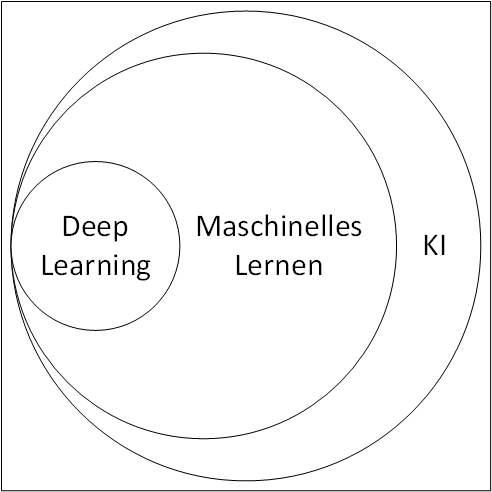
\includegraphics[width=0.45\textwidth]{img/Grafiken/Ki-ML und Deep Learning Ven.png}
        \vspace*{-10mm}
        \caption[Venn-Diagramm von KI, maschinellen Lernen und Deep Learning.]{Venn-Diagramm von KI, maschinellen Lernen und Deep Learning \cite{Goodfellow.2016}.}
        \label{fig:zusammenhangDL_ML}
    \end{center}
\end{wrapfigure}
Die Begriffe \gls{ML} und \gls{Deep Learning} stehen in einem hierarchischen Zusammenhang. \Gls{ML} umfasst alle Lernalgorithmen. Dazu zählen einfache Algorithmen wie die lineare Regression, sowie Komplexe Modelle wie sie im Bereich des \gls{Deep Learning} zu finden sind. \gls{Deep Learning} ist somit eine spezielle Art des \glsdisp{ML}{maschinellen Lernens}. Beide Teilgebiete sind in der Wissenschaft der künstlichen Intelligenz verordnet. Diesen Zusammenhang visualisiert die Abbildung \ref{fig:zusammenhangDL_ML} \cite{Goodfellow.2016, Burkov.2019}.



\gls{Deep Learning} Modelle sind aus mehreren Schichten aufgebaut. Die Schichten sind aus einfachen Algorithmen des \glsdisp{ML}{maschinellen Lernens} aufgebaut. Eine Schicht bekommt als Eingabe die Ausgabe der vorausgegangenen Schicht. Dadurch werden die meisten Modellparameter nicht durch den Datensatz direkt trainiert, sondern durch die Ausgabe der vorausgegangenen Schichten. Aus diesem Grund sind \gls{Deep Learning} Modelle auch deutlich besser in der Lage mit Rohdaten zu arbeiten, als einfachere Modell. Durch die Schichten sind sie in der Lage selbstständig \gls{Feature}[s] zu extrahieren. Eine Schicht ist aufgebaut aus Einheiten. Jede Einheit ist ein einfaches Modell, wie bspw. die lineare Regression. Durch die Schichtung solcher einfacher Modelle lassen sich sehr komplexe Muster in Daten finden. Die Abbildung \ref{fig:SimpleDL} zeigt den Aufbau eines einfachen \gls{Deep Learning} Netzwerks \cite{Burkov.2019, Goodfellow.2016}. 

\begin{figure}[htb]
    \centering
    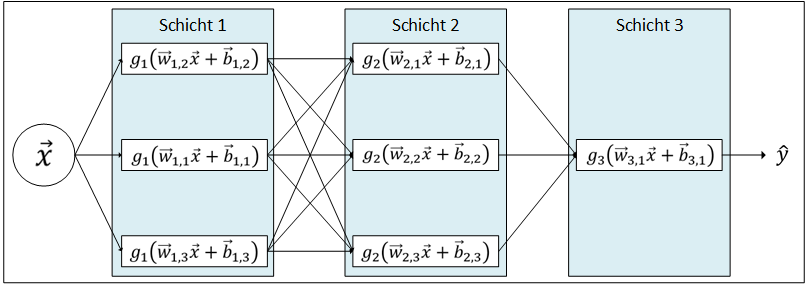
\includegraphics[width=0.9\textwidth]{img/Grafiken/Aufbau Neuronales Netz.png}
    \caption[Beispielhafter Aufbaue eines neuronalen Netzes.]{Beispielhafter Aufbaue eines neuronalen Netzes. Zu sehen sind drei verbundene Schichten. In den Schichten befinden sich Einheiten, in welchen einfache Lern-Algorithmen verwendet werden \cite{Burkov.2019}.}
    \label{fig:SimpleDL}
\end{figure}

\par
\textbf{Weitere Unterscheidungsmerkmale:}\\
Algorithmen können sich in der Menge an Daten unterscheiden, welche im Training benötigt wird um passende Modellparameter zu finden. Ebenfalls ist der Rechenaufwand für das Training von Modell zu Modell unterschiedlich hoch. Hierbei besteht auch ein Zusammenhang mit den Modellparametern. Umso mehr Modellparameter optimiert werden müssen, desto höher ist der Aufwand. Ein weiterer rechenaufwendiger Prozess ist die Suche nach optimalen \gls{Hyperparameter}[n]. Auch hier gilt, umso mehr Hyperparamter zu konfigurieren sind, desto Aufwändiger ist die Suche. Auch die Implementierung kann unterschiedlich Aufwendig sein. In der Praxis werden Algorithmen für \gls{ML} jedoch selten selst Programmiert. In den meisten fällen werden Software-\gls{Bibliothek}[en] verwendet, welche die Algorithmen implementieren. Allgemein ist es so, dass komplexe Modelle, wie im \gls{Deep Learning} höhere Anforderungen an die Datenmenge und die Rechenleistung haben, als einfache Modelle des \glsdisp{ML}{maschinellen Lernens} \cite{Burkov.2019, ShalevShwartz.2014}.


\subsection{Herausforderungen des maschinellen Lernens} \label{sec:Herausforderungen ML}
Ziel eines Modells für \gls{ML} ist es Proben zu schätzen, welche für das Modell zuvor unbekannt sind. Das bedeutet es ist nicht nur in der Lage gute Schätzungen für die Proben im Datensatz zu tätigen, mit denen es trainiert wurde, sonder es lernt zu verallgemeinern. Ein Modell, welches gute Schätzungen für bekannte und unbekannte Proben tätigen kann \glsdisp{Generalisierung}{generalisiert} gut. Ist ein Modell nicht gut im \glsdisp{Generalisierung}{generalisieren}, dann befindet es sich entweder im \gls{Overfitting} oder im \gls{Underfitting} \cite{Burkov.2019}.\dubpar

\textbf{\gls{Overfitting}:}\\
\gls{Overfitting} lässt sich als \textit{Überanpassung} übersetzen. Es tritt auf, wenn ein Modell beim training einen Datensatz zu gut lernt, so dass es nicht in der Lage ist unbekannte Proben zu schätzen. Es lernt die bekannten Proben auswendig, anstatt ein allgemeines Verständnis des Problems zu entwickeln. Für das Beispiel des Autohändlers aus dem \autoref{sec:Grundlagen ML} wird anstatt einer linearen Regression eine polynomial Regression durchgeführt, um den Verkaufswert von Autos zu schätzen. Das resultierende Modell ist in der Abbildung \ref{fig:BspOverfitting} zu sehen.

\begin{figure}[htb]
    \centering
    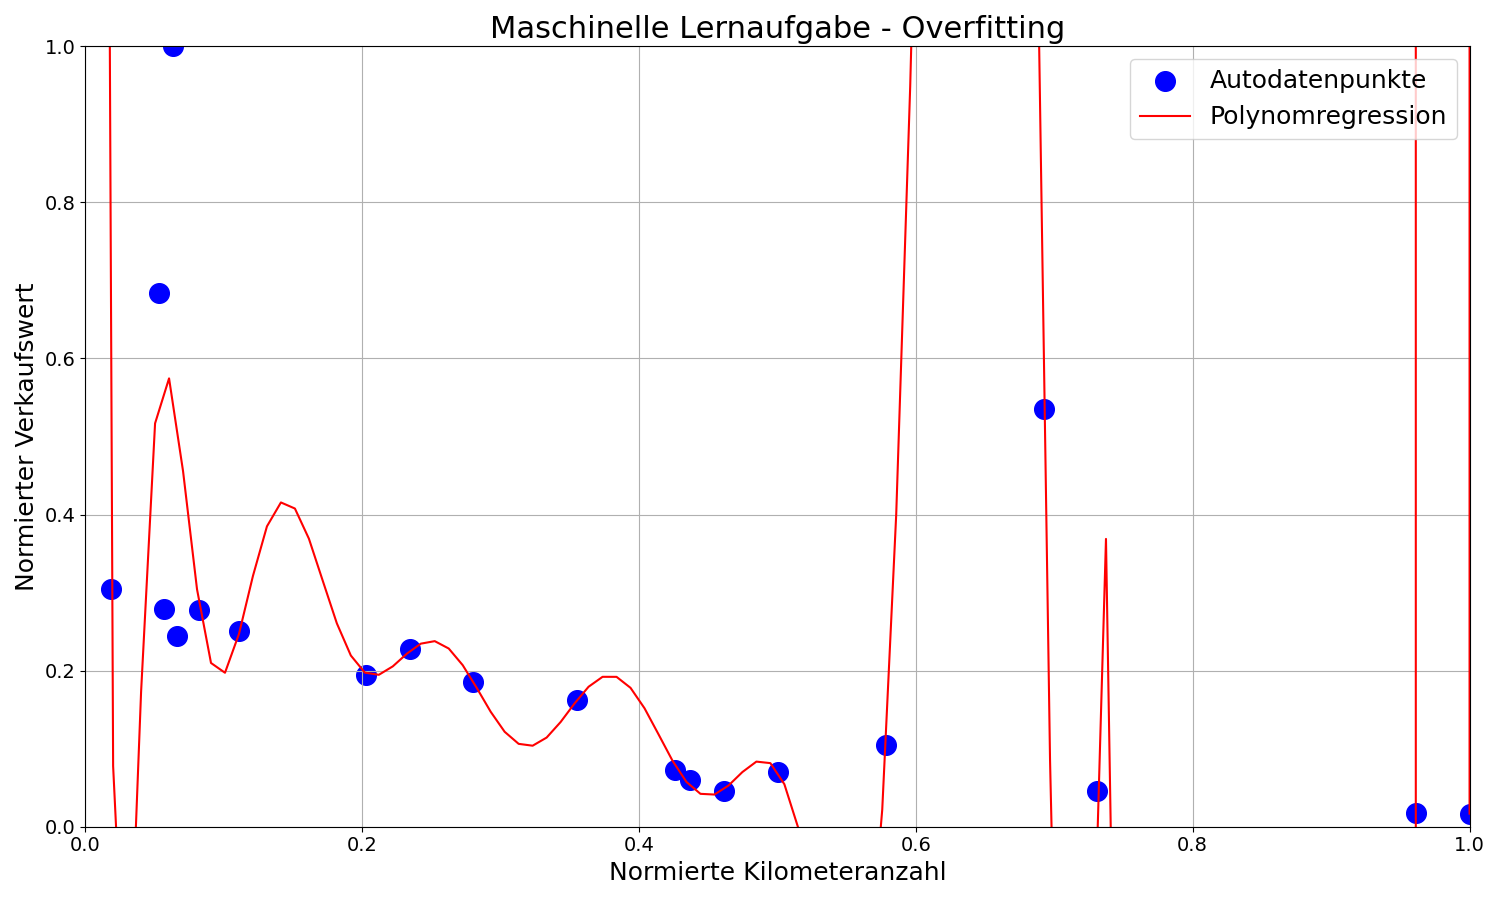
\includegraphics[width=0.9\textwidth]{img/Autohändlerbsp/Overfitting.png}
    \caption[Darstellung von Overfitting am Beispiel des Autohändlers.]{Darstellung von Overfitting am Beispiel des Autohändlers. Das Modell lernt den Datensatz im Training auswendig. Es befindet sich im Overfitting. Es ist nicht in der Lage, zuverlässig den Wert von unbekannten Autos zu schätzen.}
    \label{fig:BspOverfitting}
\end{figure}

Die Autos des Datensatzes können mit dem Modell zuverlässig geschätzt werden, für unbekannte Autos ist dies nicht möglich. Das Modell \gls{Overfitting}{overfittet}. \gls{Overfitting} kann durch eine zu hohe Modellkomplexität entstehen. Dies ist in der Abbildung \ref{fig:BspOverfitting} zu sehen. Die polynomial Regression ist zu komplex, um den einfachen Zusammenhang der Aufgabe zu modellieren. Die lineare Regression ist besser geeignet. Ein weiterer Grund für \gls{Overfitting} kann eine zu kleiner Datensatz für das Training sein. In diesem Fall hat das Modell zu wenige Beispiele, um allgemein gültige Muster der Aufgabe zu erlernen \cite{Burkov.2019, Bishop.2006, Goodfellow.2016}.\dubpar

\textbf{\gls{Underfitting}:}\\
\gls{Underfitting} ist mit \textit{Unteranpassung} zu übersetzen. Es ist das gegenteil vom \gls{Overfitting}. Anstatt das, dass Modell im Training den Datensatz zu gut lernt, lernt das Modell diesen nicht gut genug. Dadurch sind weder gute Schätzungen für bekannte Proben möglich, noch für Unbekannte. Der Autohändlers aus \autoref{sec:Grundlagen ML} macht für sein Modell die Annahme, dass jedes Auto gleich viel Wert ist unabhängig von der Anzahl der gefahrenen Kilometer. Das ist in der Abbildung \ref{fig:BspUnderfitting} zu sehen.

\begin{figure}[htb]
    \centering
    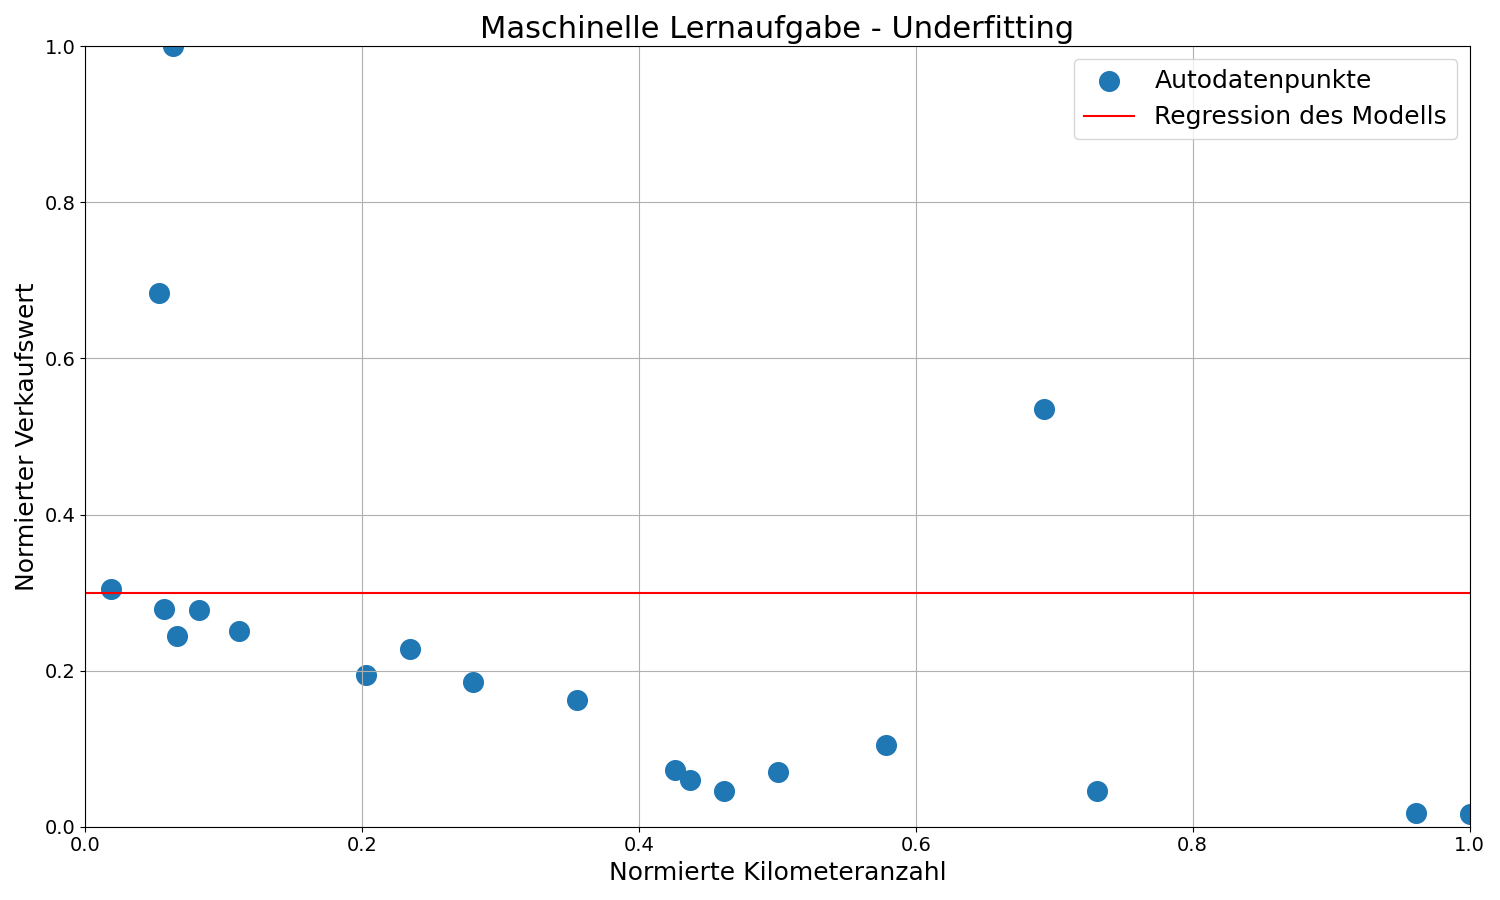
\includegraphics[width=0.9\textwidth]{img/Autohändlerbsp/Underfitting.png}
    \caption[Darstellung von Underfitting am Beispiel des Autohändlers.]{Darstellung von Overfitting am Beispiel des Autohändlers. Das Modell lernt den Datensatz im Training unzureichend. Es befindet sich im Underfitting. Es ist nicht in der Lage, zuverlässig den Wert von bekannten und unbekannten Autos zu schätzen.}
    \label{fig:BspUnderfitting}
\end{figure}

In dem Beispiel ist das Modell zwar prinzipiell überflüssig, jedoch veranschaulicht es gut, dass mit diesem Vorgehen keine guten Schätzungen für Proben jeglicher Art möglich sind. In diesem Fall liegt der Grund für das \gls{Underfitting} in einer unzureichenden Modellkomplexität. Das Modell ist zu einfach, um die Aufgabe korrekt zu modellieren. Auch eine zu geringe Anzahl an \gls{Feature}[s] oder \gls{Feature}[s], welche keine Information zu der Aufgabe besitzen, können zu \gls{Underfitting} führen. In diesem Fall hat das Modell zu wenige Information erhalten, um die Komplexität der Aufgabe vollständig zu umfassen \cite{Burkov.2019, Bishop.2006, Goodfellow.2016}.  \dubpar

\textbf{\gls{Regularisierung}:}\\
\gls{Regularisierung} ist eine Bezeichnung für Methoden, mit denen sich Algorithmen des \glsdisp{ML}{maschinellen Lernens} zwingen lassen, weniger komplexe Modelle zu lernen. Es ist nützlich um \gls{Overfitting} zu vermeiden. Ein einfaches Beispiel ist die L1 \gls{Regularisierung}. In der Formel \ref{eq:L1linReg} ist die zu optimierende \gls{Zielfunktion} der linearen Regression zu sehen. Diese wird mit einem Term für die L1 \gls{Regularisierung} ergänzt.

\begin{equation}
    \label{eq:L1linReg}
    \underset{w}{\arg\min} C\sum_{j=1}\nomvec{w}_j + \frac{1}{N} \sum_{i=1}^{N} (\hat{y}_i(\nomvec{w}, \nommat{X}_{i:}) - \nomvec{y}_i)_i^2
\end{equation}

Der Term der L1 \gls{Regularisierung} ist über den \gls{Hyperparameter} \(C\) einstellbar. Ist \(C=0\), dann finden keine \gls{Regularisierung} statt, und das Optimierungsproblem lässt sich wie in \autoref{sec:Grundlagen ML} lösen. Wird \(C\) auf einen hohen Wert gesetzt, dann wird die Lösung der Optimierung darin resultieren, dass eher kleine Werte von den  \gls{Modellparameter}[n] \(\nomvec{w}\) angenommen werden. Somit ist das resultierende Modell weniger komplex \cite{Burkov.2019}. \dubpar

\textbf{\gls{Bias}:}\\
\gls{Bias} lässt sich als \textit{Voreingenommenheit} übersetzen und beschreibt ein Modell, welches voreingenommen ist, in eine bestimmte Richtung. Der Autohändler aus \autoref{sec:Grundlagen ML} stellt fest, dass er mit seinem aktuellen Modell seine Autos fast immer unter Wert verkauft. Er sammelt neue Daten und vergleicht diese mir seinem Modell. In der Abbildung \ref{fig:BspBias} ist zu sehen, dass sein Modell einen \gls{Bias} in Richtung zu niedriger Verkaufswerte.

\begin{figure}[htb]
    \centering
    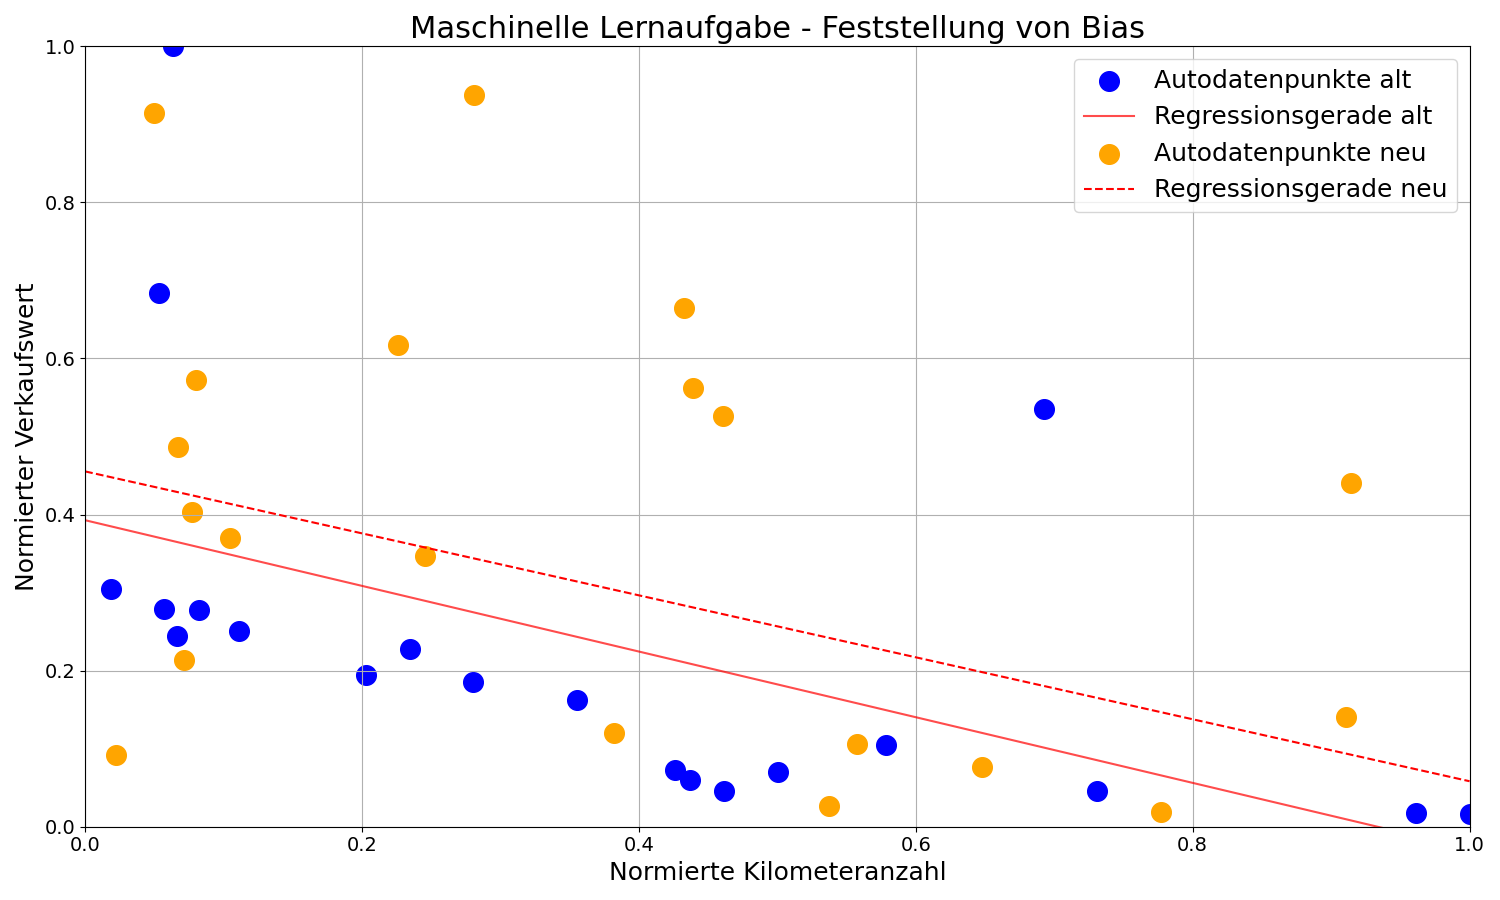
\includegraphics[width=0.9\textwidth]{img/Autohändlerbsp/Feststellung von Bias.png}
    \caption[Darstellung von Bias am Beispiel des Autohändlers.]{Darstellung von Bias am Beispiel des Autohändlers. Durch die neuen Daten fällt auf, dass das Modell die Verkaufswerte der Autos zu niedrig schätzt. Insgesamt scheint die lineare Regression  \gls{Underfitting} zu verursachen.}
    \label{fig:BspBias}
\end{figure}

Ein solcher \gls{Bias} kann verschieden Ursachen haben. Z.B. kann es sein, dass nicht alle Faktoren, welcher die Aufgabe beeinflussen mit in das Modell aufgenommen wurden. Der Verkaufswert von Autos kann bspw. von der jahreszeit abhängen. Der Autohändler berücksichtigt in seinem Modell keine saisonale Abhängigkeit. Auch fehlende Varianz im Datensatz kann \gls{Bias} verursachen. Der Autohändler stellt fest, dass in seinem Datensatz nur Autos von zwei Marken vorhanden sind. Andere Automarken erzielen höhere Verkaufswerte. Ihm fehlt es an Varianz in seinen Proben, um die Aufgabe korrekt zu modellieren. Von den beiden Automarken in seinem Datensatz stellt die ein preiswertere Autos her, die Andere ist für Luxusautos bekannt. Jedoch  befinden sich im Datensatz nur drei Proben von der Luxusmarke. Der Datensatz ist somit unbalanciert. Das kenn ebenfalls \gls{Bias} verursachen. Das Modell tendiert dazu, die Eigenschaften des preiswerten Herstellers zu lernen, da dieser deutlich stärker im Datensatz vertreten ist. Auch \gls{Regularisierung} kann einen \gls{Bias} verursachen, in dem durch die reduzierte Komplexität eine unbeabsichtigte Voreingenommenheit entsteht. \gls{Bias} kann die Schätzungen eines Modells verzerren, was die Zuverlässigkeit einschränkt. Es ist oftmals schwierig zu erkennen, wo \gls{Bias} in ein Modell eingeführt wird. Aufmerksamkeit beim Aufbau eines Modells bezüglich \gls{Bias} sollte stehst vorhanden sein. \gls{Bias} muss jedoch nicht nur negativ sein. Gezielt eingesetzt kann er nützlich sein, um Modelle zu vereinfachen und eine bessere \gls{Generalisierung} ermöglichen. Der Autohändler möchte sich z.B. auf SUVs spezialisieren. Aus diesem Grund benutzt er für sein neues Modell nur Proben von SUVs. Dadurch besitzt sein Datensatz einen \gls{Bias} durch geringe Varianz bezüglich der Bauart der Autos. Jedoch ist das Modell angepasster an seinen speziellen Fall und sollte für Verkaufswerte von SUVs gut \glsdisp{Generalisierung}{generalisieren} können \cite{Burkov.2019, Goodfellow.2016, Mehrabi.2019}. \dubpar

\textbf{\gls{Leakage}:}\\
Auf deutsch ist \gls{Leakage} mit \textit{Datenleck} zu übersetzen. Es sagt aus, dass sich Daten irgendwo befinden, wo sie eigentlich nicht seien sollten. Das kann im \glsdisp{ML}{maschinellen Lernen} problematisch werden. Um Modelle zu evaluieren, wird die Performance auf unbekannten Proben betrachte. Passiert es jedoch, dass sich unter die Testproben auch bereits bekannte Proben mischen wird dies als \gls{Leakage} bezeichnet. In diesem Fall führt \gls{Leakage} dazu, dass das Modell übermäßig Optimistische Bewertungsergebnisse erzielt. \gls{Leakage} wird in den meisten Fällen vom Anwender verursacht und lässt sich durch Aufmerksamkeit vermeiden \cite{Zheng.2015}.


\subsection{Sequenzen im maschinellen Lernen} \label{sec:sequenzen ML}
Eine Sequenz ist eine Menge von Daten, die in einer geordneten Reihenfolge zu einander stehen. Für moderne Modelle im \glsdisp{ML}{maschinellen Lernen} besitzen sie hohe Relevanz, da viele Aufgaben in Sequenzen strukturiert sind. Dazu zählen Zeitreihen, wie z.B. Aktienkurse oder Wetterdaten, aber auch Sprache und Text sind Sequenzen. Die Fähigkeit Sequenzen zu verstehen ist essentiell für Modelle, um zeitliche Muster zu erkennen und Kontext zu verstehen. \par

Währende den Anfängen des \glsdisp{ML}{maschinellen Lernens} stand Sequenzverständnis nicht im Fokus. Aus diesem Grund besitzen die einfacheren Modelle diese Fähigkeit nicht. Sie sind nicht in der Lage Reihenfolgen in Daten zu berücksichtigen. Komplexere Modelle wie sie im \gls{Deep Learning} vorkommen besitzen diese Fähigkeit. Solche Modelle besitzen eine Art Gedächtnis, was ihr Sequenzverständnis ermöglicht. Ebenfalls ist die Fähigkeit Rohdaten zu verarbeiten hier von Vorteil, da sie eigenständig Muster in Sequenzen finden.\par

Auch wenn Sequenzen nicht direkt dazu in der Lage sind Sequenzen zu verstehen, so gibt es dennoch Ansätze wie sich Sequenzen verarbeiten lassen. Z.B. lassen sich \gls{Feature} [s] extrahieren, welche versuchen die wichtigsten Eigenschaften der Sequenzen zu komprimieren. Solche \gls{Feature}[s] können Mittelwerte sein, die Standard Abweichung oder Maxima und Minima. Die Sequenz aus mehreren Datenpunkten wird zu einem einzelnen Datenpunkt komprimiert. Eine weitere Option sind Distanzmetriken, um die Ähnlichkeit von Sequenzen zu messen. Für Zeitreihen ist dies z.B. mit dem Dynamik Time Warping möglich. Damit lässt sich die Distanz zwischen zwei Zeitreihen bestimmen. Über dieses Ähnlichkeitsmaß ist anschließend ein Clustering möglich. Über solche Methoden sind auch einfachere Modelle für Aufgaben anwendbar, bei denen Sequenzen geschätzt werden sollen \cite{Nielsen.2020}.